\section{Results and Analysis}\label{sec:results}

Figure~\ref{fig:forest} shows the HOTA difference between each host with
\scl{} and the host alone for every tested cell. The next subsections give
the baseline comparison for each part of the evaluation, in the order of the
three expectations of Sect.~\ref{sec:setup}: well-matched trackers, trackers
that do not fit their detector, and systems not seen during design.

\begin{figure}[t]
\centering
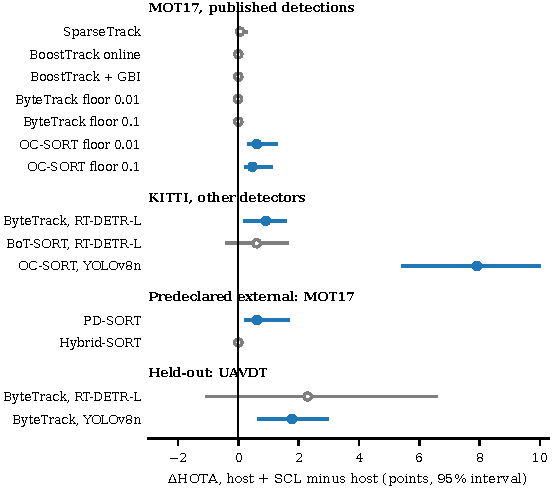
\includegraphics[width=\columnwidth]{fig3_forest_col.pdf}
\caption{Difference in HOTA (host with \scl{} minus host alone) with
95\% paired-bootstrap interval for every tested cell. Filled blue circles:
interval above zero; open gray circles: interval contains zero, or identical
output}
\label{fig:forest}
\end{figure}

\subsection{Results across trackers}\label{sec:tracker}
Table~\ref{tab:mot17} compares the development trackers with their hosts on
MOT17. The two-stage trackers with well-matched detections stayed at the
accuracy of their hosts. BoostTrack, online and with GBI, and
ByteTrack at floor 0.1 gave identical output, and ByteTrack at floor 0.01 and
SparseTrack stayed within 0.06 HOTA points of their hosts ($-0.014$ and
$+0.055$). This is the
self-limiting behavior of the clean mode (Sect.~\ref{sec:regimes}), which
the earlier design did not have (Table~\ref{tab:prior}).

The single-stage OC-SORT improved at both emission floors. Its HOTA rose by
0.61 points ($[+0.36,+1.24]$) at floor 0.01 and by 0.46 points
($[+0.27,+1.09]$) at floor 0.1, and its MOTA by 1.27 and 1.26 points. HOTA
was higher on 7 of 7 sequences in both settings (Fig.~\ref{fig:perseq}). The
gain comes from the continuation rescue. OC-SORT drops every detection
below its single threshold, and the layer passes it the foreground candidates
that continue a track that would otherwise stay unmatched.

\begin{table}[t]
\caption{Baseline comparison of the development trackers on MOT17 val-half
(published YOLOX-X detections). Paper: number reported by the tracker's
authors. Host: published tracker alone (our reproduction). $\Delta$: host with
\scl{} minus host, with 95\% paired-bootstrap interval (10,000
resamples, seed 42); bold intervals exclude zero. The floor is the lowest
detector score emitted.}
\label{tab:mot17}
\centering\footnotesize
\setlength{\tabcolsep}{4pt}
\begin{tabular}{@{}lrrl@{}}
\toprule
Metric & Paper & Host & $\Delta$ [95\% CI]\\
\midrule
\multicolumn{4}{@{}l}{\textit{SparseTrack} \cite{liu2025sparsetrack}}\\
\quad HOTA & 69.2 & 68.88 & $+0.06$ [$-0.01$, $+0.25$]\\
\quad MOTA & 76.8 & 77.85 & $+0.08$ [$-0.03$, $+0.30$]\\
\quad IDF1 & 81.4 & 81.97 & $+0.16$ [$-0.02$, $+0.70$]\\
\multicolumn{4}{@{}l}{\textit{BoostTrack, online} \cite{stanojevic2024boosttrack}}\\
\quad HOTA & 68.37 & 68.49 & 0 (identical)\\
\quad MOTA & 75.56 & 75.50 & 0 (identical)\\
\quad IDF1 & 81.35 & 81.41 & 0 (identical)\\
\multicolumn{4}{@{}l}{\textit{BoostTrack, + GBI} \cite{stanojevic2024boosttrack}}\\
\quad HOTA & 71.33 & 71.72 & 0 (identical)\\
\quad MOTA & 80.55 & 81.03 & 0 (identical)\\
\quad IDF1 & 83.84 & 84.16 & 0 (identical)\\
\multicolumn{4}{@{}l}{\textit{ByteTrack, floor 0.01} \cite{zhang2022bytetrack}}\\
\quad HOTA & -- & 67.70 & $-0.014$ [$-0.058$, $+0.009$]\\
\quad MOTA & 76.6 & 77.60 & $+0.06$ [$-0.15$, $+0.34$]\\
\quad IDF1 & 79.3 & 79.47 & $-0.031$ [$-0.135$, $+0.035$]\\
\multicolumn{4}{@{}l}{\textit{ByteTrack, floor 0.1} \cite{zhang2022bytetrack}}\\
\quad HOTA & -- & 67.70 & 0 (identical)\\
\quad MOTA & 76.6 & 77.60 & 0 (identical)\\
\quad IDF1 & 79.3 & 79.47 & 0 (identical)\\
\multicolumn{4}{@{}l}{\textit{OC-SORT, floor 0.01} \cite{cao2023ocsort}}\\
\quad HOTA & 66.5 & 66.43 & {\boldmath $+0.61$ [$+0.36$, $+1.24$]}\\
\quad MOTA & 74.9 & 74.67 & {\boldmath $+1.27$ [$+0.17$, $+3.01$]}\\
\quad IDF1 & 77.7 & 78.05 & $+0.66$ [$-0.25$, $+1.60$]\\
\multicolumn{4}{@{}l}{\textit{OC-SORT, floor 0.1} \cite{cao2023ocsort}}\\
\quad HOTA & 66.5 & 66.44 & {\boldmath $+0.46$ [$+0.27$, $+1.09$]}\\
\quad MOTA & 74.9 & 74.67 & {\boldmath $+1.26$ [$+0.37$, $+3.34$]}\\
\quad IDF1 & 77.7 & 78.05 & {\boldmath $+0.287$ [$+0.003$, $+0.838$]}\\
\bottomrule
\end{tabular}
\end{table}


\begin{figure}[t]
\centering
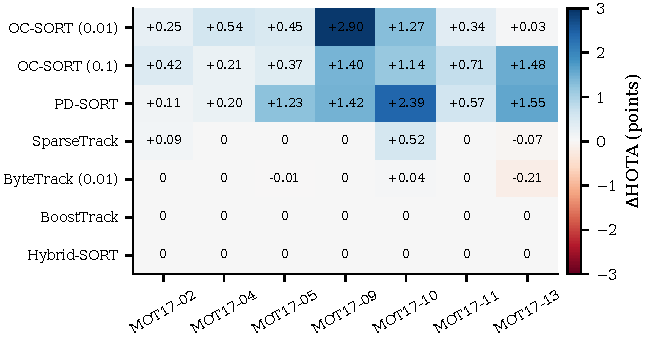
\includegraphics[width=\columnwidth]{fig4_per_sequence.pdf}
\caption{Per-sequence HOTA differences (host with \scl{} minus host
alone) on MOT17 val-half for the development and predeclared trackers}
\label{fig:perseq}
\end{figure}

\subsection{Results with other detectors}\label{sec:detector}
Table~\ref{tab:kitti} reports the KITTI results with the two other detectors. With
the noisy RT-DETR-L detector, the two-stage trackers gained in MOTA and IDF1.
ByteTrack gained 5.98 MOTA points ($[+1.16,+9.94]$), 3.87 IDF1 points, and
0.91 HOTA points ($[+0.22,+1.55]$). BoT-SORT gained 7.86 MOTA points
($[+2.21,+13.44]$) and 3.10 IDF1 points. With YOLOv8n, the single-stage
OC-SORT gained 7.91 HOTA points ($[+5.47,+9.98]$), 9.40 MOTA points, and 9.60
IDF1 points.

\begin{table}[t]
\caption{Baseline comparison under a detector change on KITTI tracking
training (official HOTA, car and pedestrian averaged). Host: published
tracker alone with the same detections. $\Delta$: host with \scl{}
minus host, with 95\% paired-bootstrap interval; bold intervals exclude zero.}
\label{tab:kitti}
\centering\footnotesize
\setlength{\tabcolsep}{4pt}
\begin{tabular}{@{}lrl@{}}
\toprule
Metric & Host & $\Delta$ [95\% CI]\\
\midrule
\multicolumn{3}{@{}l}{\textit{ByteTrack} \cite{zhang2022bytetrack}\textit{, RT-DETR-L}}\\
\quad HOTA & 50.73 & {\boldmath $+0.91$ [$+0.22$, $+1.55$]}\\
\quad MOTA & 47.27 & {\boldmath $+5.98$ [$+1.16$, $+9.94$]}\\
\quad IDF1 & 64.98 & {\boldmath $+3.87$ [$+1.67$, $+5.06$]}\\
\multicolumn{3}{@{}l}{\textit{BoT-SORT} \cite{aharon2022botsort}\textit{, RT-DETR-L} (20 sequences)}\\
\quad HOTA & 53.91 & $+0.61$ [$-0.39$, $+1.61$]\\
\quad MOTA & 48.25 & {\boldmath $+7.86$ [$+2.21$, $+13.44$]}\\
\quad IDF1 & 67.74 & {\boldmath $+3.10$ [$+1.00$, $+4.57$]}\\
\multicolumn{3}{@{}l}{\textit{OC-SORT} \cite{cao2023ocsort}\textit{, YOLOv8n}}\\
\quad HOTA & 36.27 & {\boldmath $+7.91$ [$+5.47$, $+9.98$]}\\
\quad MOTA & 33.99 & {\boldmath $+9.40$ [$+1.10$, $+12.30$]}\\
\quad IDF1 & 50.46 & {\boldmath $+9.60$ [$+5.61$, $+12.16$]}\\
\bottomrule
\end{tabular}
\end{table}


\subsection{Results under shifted detector scores}\label{sec:shift}
Table~\ref{tab:shift} and Fig.~\ref{fig:shift} show the trackers under the
four score transforms. Halving the scores reduced ByteTrack (official setting)
and OC-SORT to 0 HOTA, because no detection reached their thresholds. With the
layer they reached 66.17 and 66.72. Cubing reduced them to 60.92 and 58.34,
and the layer restored them to 65.81 and 66.60. BoostTrack rose from 61.33 to
64.84 under cubing. With temperature $T=2$, the layer raised ByteTrack and
OC-SORT by 1.11 and 1.24 points. The library setting of ByteTrack, whose low
thresholds already accept the changed scores, stayed within 0.14 points in all
four transforms. Over the 14 conditions, the layer raised HOTA significantly
in 7 and lowered it significantly in none.

\begin{table}[t]
\caption{Baseline comparison under shifted detector scores on MOT17 val-half
(HOTA). The detector scores are transformed before the tracker, whose
published thresholds stay fixed; $T$ is a logit temperature, $\sigma(z/T)$.
Host: published tracker alone. $\Delta$: with \scl{} minus host,
with 95\% paired-bootstrap interval (10,000 resamples, seed 42). Bold
intervals exclude zero. Emission floor 0.01 (BoostTrack 0.1).}
\label{tab:shift}
\centering\footnotesize
\setlength{\tabcolsep}{4pt}
\begin{tabular}{@{}lrrl@{}}
\toprule
Transform & Host & + \scl{} & $\Delta$HOTA\\
\midrule
\multicolumn{4}{@{}l}{\textit{ByteTrack, official setting} \cite{zhang2022bytetrack}}\\
\quad $s^3$ & 60.92 & 65.81 & {\boldmath $+4.89$ [$+2.60$, $+13.69$]}\\
\quad $0.5\,s$ & 0.00 & 66.17 & {\boldmath $+66.17$ [$+49.32$, $+75.40$]}\\
\quad $T=2$ & 65.84 & 66.95 & {\boldmath $+1.11$ [$+0.35$, $+3.87$]}\\
\quad $T=0.5$ & 67.30 & 67.29 & $-0.009$ [$-0.051$, $+0.005$]\\
\multicolumn{4}{@{}l}{\textit{ByteTrack, library setting} \cite{zhang2022bytetrack}}\\
\quad $s^3$ & 66.31 & 66.31 & $-0.006$ [$-0.384$, $+0.383$]\\
\quad $0.5\,s$ & 66.61 & 66.48 & $-0.14$ [$-0.66$, $+0.14$]\\
\quad $T=2$ & 63.97 & 63.97 & 0 (identical)\\
\quad $T=0.5$ & 66.53 & 66.52 & $-0.006$ [$-0.029$, $+0.001$]\\
\multicolumn{4}{@{}l}{\textit{OC-SORT} \cite{cao2023ocsort}}\\
\quad $s^3$ & 58.34 & 66.60 & {\boldmath $+8.26$ [$+5.86$, $+16.81$]}\\
\quad $0.5\,s$ & 0.00 & 66.72 & {\boldmath $+66.72$ [$+50.32$, $+75.56$]}\\
\quad $T=2$ & 65.99 & 67.22 & {\boldmath $+1.24$ [$+0.52$, $+3.42$]}\\
\quad $T=0.5$ & 66.61 & 67.06 & $+0.45$ [$-0.01$, $+0.97$]\\
\multicolumn{4}{@{}l}{\textit{BoostTrack, online} \cite{stanojevic2024boosttrack}}\\
\quad $s^3$ & 61.33 & 64.84 & {\boldmath $+3.51$ [$+0.85$, $+13.28$]}\\
\quad $T=2$ & 67.59 & 67.59 & 0 (identical)\\
\bottomrule
\end{tabular}
\end{table}


\begin{figure*}[t]
\centering
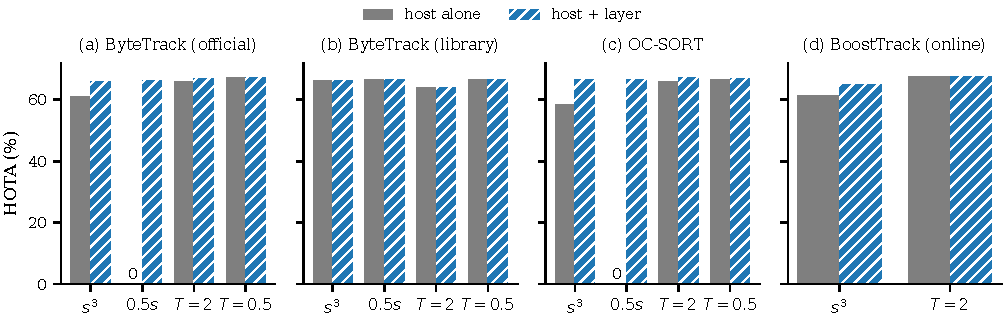
\includegraphics[width=0.9\textwidth]{fig5_calibration_shift.pdf}
\caption{Shifted detector scores on MOT17 val-half: HOTA of each published
tracker with its published thresholds, alone and with \scl{}, after
four monotone transforms of the detector scores ($s^3$, $0.5\,s$, and
temperatures $T=2$ and $T=0.5$). (a) ByteTrack, official setting;
(b) ByteTrack, library setting; (c) OC-SORT; (d) BoostTrack, online. Hatched bars:
host with \scl{}}
\label{fig:shift}
\end{figure*}

\subsection{Comparison with adaptive-threshold methods}\label{sec:baselines}
A simpler way to follow the detector scores is to set the tracker's
thresholds from them directly. Two such baselines were built on the same
input and with the same window of the last 10 frames. They set the tracker's
matching and birth thresholds in every frame to the first or the second Otsu
split of the recent logits, $t_1$ or $t_2$, and pass the scores unchanged,
without the mode decision, the new scores, or the rescue.
Table~\ref{tab:baselines} compares them with \scl{} on KITTI, for OC-SORT
with YOLOv8n and for both trackers under halved scores. \scl{} reached the
highest HOTA in all three cells, 2.2 to 8.6 points above the two baselines,
and its paired-bootstrap intervals against the $t_2$ baseline lie
above zero in every cell. Adaptive thresholds alone therefore do not explain
the gains; the other parts of the layer add to them.

\emph{Comparison with a published method.} ACT \cite{act2026adaptive} sets the
high and low thresholds of a two-stage tracker in every frame from the first
quartile and the number of the current scores, using fixed score levels. It
was run with its published parameters on the same detections, for ByteTrack
and, with its high threshold as the single threshold, for OC-SORT. Under
halved scores, \scl{} reached higher HOTA than ACT with both trackers: 51.78
against 49.77 with ByteTrack and RT-DETR-L (difference $+2.01$,
[$+0.01$, $+4.76$]) and 46.30 against 36.24 with OC-SORT and YOLOv8n
(difference $+10.06$, [$+6.88$, $+12.01$]). The levels of ACT are fixed
scores, so they do not move when all scores shift, while the splits of
\scl{} are computed on the scores themselves.

\emph{Contribution of each part.} Removing one part of the frozen \scl{} at
a time shows where the gains come from, on the KITTI cells. Without the
continuation rescue, the HOTA of OC-SORT fell by 3.34 points with YOLOv8n and
by 1.16 points under halved scores. Using the clean mode in every frame,
that is, without the mode decision, lowered HOTA by 0.90 points
for ByteTrack with RT-DETR-L and by 2.40 and 2.44 points for the two trackers
under halved scores. Without the new scores of the noisy mode, HOTA fell by
1.67 and 0.61 points under halved scores.

\begin{table*}[t]
\caption{HOTA of \scl{} and of two simple adaptive-threshold baselines on KITTI
tracking training (official HOTA, car and pedestrian averaged). Adaptive $t_1$,
$t_2$: the tracker's matching and birth thresholds are set in every frame to the
first or second Otsu split of the logits of the last 10 frames, and the scores
are passed unchanged. $\Delta$: \scl{} minus the adaptive $t_2$ baseline, with
95\% paired-bootstrap interval; bold intervals exclude zero.}
\label{tab:baselines}
\centering\footnotesize
\setlength{\tabcolsep}{4pt}
\begin{tabular}{@{}lrrrrl@{}}
\toprule
Cell & Host & Adapt.\ $t_1$ & Adapt.\ $t_2$ & \scl{} & $\Delta$ [95\% CI]\\
\midrule
\twol{OC-SORT, YOLOv8n}{} & 36.27 & 39.97 & 41.09 & 44.17 & {\boldmath $+3.09$ [$+2.00$, $+4.03$]}\\
\addlinespace[4pt]
\twol{ByteTrack, RT-DETR-L,}{halved scores} & 49.50 & 49.58 & 49.50 & 51.78 & {\boldmath $+2.29$ [$+0.28$, $+4.96$]}\\
\addlinespace[4pt]
\twol{OC-SORT, YOLOv8n,}{halved scores} & 0.00 & 37.68 & 43.56 & 46.30 & {\boldmath $+2.74$ [$+1.32$, $+3.34$]}\\
\bottomrule
\end{tabular}
\end{table*}


\subsection{Results on external trackers}\label{sec:external}
Table~\ref{tab:external} gives the two predeclared external systems. PD-SORT
\cite{wang2025pdsort} was reproduced exactly as in the authors' released
output. With \scl{}, its HOTA rose by 0.61 points ($[+0.27,+1.65]$), its
MOTA by 1.13 points ($[+0.27,+3.03]$), and its IDF1 by 0.82 points
($[+0.43,+1.94]$), with higher HOTA on 7 of 7 sequences
(Fig.~\ref{fig:perseq}). FN fell by 1,291, and FP rose by 681. PD-SORT is a single-stage tracker, and its gain comes from the same
step as for OC-SORT; unlike OC-SORT, it was not seen during design.
Hybrid-SORT \cite{yang2024hybridsort}, a two-stage tracker, gave identical
output, as predicted before the run.

\begin{table}[t]
\caption{Baseline comparison on the predeclared external systems (MOT17
val-half, authors' released detections), each evaluated once with the frozen
\scl{}. Paper: number reported by the authors (for PD-SORT, their released
output). Host: published tracker alone (our reproduction). Reproduction class
against the authors' number (EXACT: $|\Delta\mathrm{HOTA}|\le0.2$; CLOSE:
$\le1.0$ with a documented, untuned cause). $\Delta$: host with \scl{} minus
host, with 95\% paired-bootstrap interval; bold intervals exclude zero.}
\label{tab:external}
\centering\footnotesize
\setlength{\tabcolsep}{4pt}
\begin{tabular}{@{}lrrl@{}}
\toprule
Metric & Paper & Host & $\Delta$ [95\% CI]\\
\midrule
\multicolumn{4}{@{}l}{\textit{PD-SORT} \cite{wang2025pdsort}\textit{, EXACT}}\\
\quad HOTA & 68.01 & 68.01 & {\boldmath $+0.61$ [$+0.27$, $+1.65$]}\\
\quad MOTA & 75.19 & 75.19 & {\boldmath $+1.13$ [$+0.27$, $+3.03$]}\\
\quad IDF1 & 81.03 & 81.03 & {\boldmath $+0.82$ [$+0.43$, $+1.94$]}\\
\multicolumn{4}{@{}l}{\textit{Hybrid-SORT} \cite{yang2024hybridsort}\textit{, CLOSE}}\\
\quad HOTA & 67.1 & 66.70 & 0 (identical)\\
\quad MOTA & 75.8 & 75.52 & 0 (identical)\\
\quad IDF1 & 78.0 & 77.56 & 0 (identical)\\
\bottomrule
\end{tabular}
\end{table}


\subsection{Results on held-out aerial data}\label{sec:visdrone}
Table~\ref{tab:visdrone} gives the held-out UAVDT test split. \scl{} raised the HOTA of the YOLOv8n stream by 1.77 points
($[+0.70,+2.94]$) and its IDF1 by 3.97 points ($[+1.88,+6.17]$), and
identity switches fell by 45\%. With RT-DETR-L, the host produced many false
positives (MOTA 3.29); with \scl{}, its MOTA rose by 24.70 points
($[+10.06,+51.08]$) and its IDF1 by 5.74 points ($[+0.13,+13.11]$): false
positives fell by 58\% and identity switches by 56\%. HOTA did not fall with either
detector.

\begin{table}[t]
\caption{Baseline comparison on the held-out UAVDT test split (20 aerial
sequences, not used during design), evaluated once with the frozen \scl{}. Host: ByteTrack alone with its published setting. $\Delta$: host
with \scl{} minus host, with 95\% paired-bootstrap interval; bold intervals
exclude zero.}
\label{tab:visdrone}
\centering\footnotesize
\setlength{\tabcolsep}{4pt}
\begin{tabular}{@{}lrl@{}}
\toprule
Metric & Host & $\Delta$ [95\% CI]\\
\midrule
\multicolumn{3}{@{}l}{\textit{ByteTrack, RT-DETR-L} \cite{zhang2022bytetrack,zhao2024rtdetr}}\\
\quad HOTA & 40.07 & $+2.30$ [$-1.05$, $+6.55$]\\
\quad MOTA & 3.29 & {\boldmath $+24.70$ [$+10.06$, $+51.08$]}\\
\quad IDF1 & 48.59 & {\boldmath $+5.74$ [$+0.13$, $+13.11$]}\\
\multicolumn{3}{@{}l}{\textit{ByteTrack, YOLOv8n} \cite{zhang2022bytetrack,jocher2023yolov8}}\\
\quad HOTA & 29.05 & {\boldmath $+1.77$ [$+0.70$, $+2.94$]}\\
\quad MOTA & 16.27 & $+1.02$ [$-1.06$, $+2.86$]\\
\quad IDF1 & 34.52 & {\boldmath $+3.97$ [$+1.88$, $+6.17$]}\\
\bottomrule
\end{tabular}
\end{table}


\subsection{Running time}\label{sec:latency}
\label{sec:latency-setup}Running time was measured after the freeze on one cloud machine with a 4-vCPU
Intel Xeon processor at 2.10 GHz, 15 GB of memory, and no graphics processing unit (GPU). A live YOLOv8n
detector (32-bit floats, 736 pixels, batch 1) feeds ByteTrack on three KITTI
tracking sequences (0001, 0009, and 0019). Both runs use the same frames
one after the other, and the first ten frames of each sequence are excluded,
which leaves 2,279 timed frames per run. The time of the layer includes the
motion cue, the per-frame step, and saving the tracker output.

Table~\ref{tab:runtime} and Fig.~\ref{fig:runtime} compare the time per frame
of the host pipeline with and without \scl{}. \scl{} took 2.95 ms per
frame on average and 4.39 ms at the 95th percentile, including the
phase-correlation motion cue. The total time rose from 57.85 to 60.44 ms
per frame, by 4.5\%. The tracker became faster, from 2.04 to 1.43 ms per
frame, because it received fewer candidates. The detector takes most of each
frame, about 42 ms, so the layer adds only a small part of the total time.

\begin{table}[t]
\caption{Baseline comparison of the per-frame time on a 4-vCPU Intel Xeon
(2.10 GHz, no GPU) with a live YOLOv8n detector (736 pixels) and ByteTrack on
three KITTI sequences (2,279 timed frames per arm). Host alone: the same
pipeline without \scl{}. Mean / 95th percentile in milliseconds.}
\label{tab:runtime}
\centering\footnotesize
\setlength{\tabcolsep}{4pt}
\begin{tabular}{@{}lcc@{}}
\toprule
Stage & Host alone & Host + \scl{}\\
\midrule
Frame decode & 13.88 / 16.21 & 13.88 / 16.51\\
Detector (YOLOv8n, 736 px) & 41.91 / 58.41 & 42.17 / 59.43\\
\scl{} & -- & 2.95 / 4.39\\
Tracker (ByteTrack) & 2.04 / 3.57 & 1.43 / 2.64\\
End to end & 57.85 / 76.35 & 60.44 / 80.78\\
\bottomrule
\end{tabular}
\end{table}


\begin{figure}[t]
\centering
\begin{tikzpicture}
\begin{axis}[
  xbar stacked,
  /pgf/bar width=10pt,
  width=0.8\columnwidth,
  height=3.9cm,
  xmin=0, xmax=72,
  clip=false,
  ymin=-0.6, ymax=1.6,
  ytick={0,1},
  yticklabels={Host + \scl{}, Host alone},
  xlabel={Mean time per frame (ms)},
  axis x line*=bottom,
  axis y line*=left,
  tick label style={font=\scriptsize},
  label style={font=\scriptsize},
  legend style={at={(0.5,1.04)}, anchor=south, legend columns=2,
    font=\scriptsize, draw=none, /tikz/every even column/.append style={column sep=6pt}},
  legend cell align=left,
]
\addplot[fill=black!20, draw=black!50] coordinates {(13.88,1) (13.88,0)};
\addplot[fill=black!45, draw=black!60] coordinates {(41.91,1) (42.17,0)};
\addplot[fill=blue!65, draw=blue!80, postaction={pattern=crosshatch dots, pattern color=white}] coordinates {(0,1) (2.95,0)};
\addplot[fill=black!75, draw=black!85] coordinates {(2.04,1) (1.43,0)};
\legend{Frame decode, Detector (YOLOv8n), \scl{}, Tracker (ByteTrack)}
\node[anchor=west, font=\scriptsize] at (axis cs:58.6,1) {57.85 ms};
\node[anchor=west, font=\scriptsize] at (axis cs:61.2,0) {60.44 ms};
\end{axis}
\end{tikzpicture}

\caption{Mean per-frame time by stage for the host pipeline alone and with
\scl{} (4-vCPU Intel Xeon, no GPU). The labels give the measured
end-to-end time}
\label{fig:runtime}
\end{figure}
